% Created 2018-04-10 Tue 12:52
\documentclass[titlepage]{article}
\usepackage[utf8]{inputenc}
\usepackage[T1]{fontenc}
\usepackage{graphicx}
\usepackage{grffile}
\usepackage{longtable}
\usepackage{wrapfig}
\usepackage{rotating}
\usepackage[normalem]{ulem}
\usepackage{amsmath}
\usepackage{textcomp}
\usepackage{amssymb}
\usepackage{capt-of}
\usepackage{hyperref}
\usepackage{mathptmx}
\author{Cai AoAhen(U1522078L) \\
EEE \\
}
\date{Apr. 8, 2018 \\
}
\title{
\includegraphics[width=\textwidth]{img/NTU.png} \\
[2\baselineskip] Assignment ON \\
EE4478 Digital video processing\\
Tutorial 2-11 \\
[3\baselineskip]}
\hypersetup{
 pdfauthor={Cai AoAhen(U1522078L) \\
EEE \\
},
 pdftitle={
\includegraphics[width=\textwidth]{img/NTU.png} \\
[2\baselineskip] Assignment ON \\
EE4478 Digital video processing\\
Tutorial 2-11 \\
[3\baselineskip]},
 pdfkeywords={},
 pdfsubject={},
 pdfcreator={Emacs 27.0.50 (Org mode 9.1.9)},
 pdflang={English}}
\begin{document}

\maketitle
\tableofcontents

\listoffigures
\listoftables

\newpage

\section{Assignment 5 Discrete Cosine Transform (DCT)}
\label{sec:orgc723f27}

I use RGB 3 layer to calculate.
\begin{verbatim}
clear all;
close all;
clc;
raw_input_img=imread('lena512c.jpg');
redChannel = dct2(raw_input_img(:, :, 1));
greenChannel = dct2(raw_input_img(:, :, 2));
blueChannel = dct2(raw_input_img(:, :, 3));
input_img = cat(3, redChannel, greenChannel, blueChannel);
QP=10;
quantized_img=round(input_img./QP);
rec_img=quantized_img.*QP;
n_img = cat(3,idct2(rec_img(:, :, 1)),idct2(rec_img(:, :, 2)),idct2(rec_img(:, :, 3)));
error= double(raw_input_img) - n_img;
subplot(1,4,1);
imshow(raw_input_img);
title('Original image');
subplot(1,4,2);
imshow(uint8(n_img));
title(['Reconstructed image (QP=' num2str(QP) ')']);
subplot(1,4,3);
imshow(error);
title('quantization error')
\end{verbatim}

The output shown in below and I find that the higher the quant level the quality of the imgae will drop and more color appear in error. And quantiztion error contain all the high frequent infomation.

\begin{figure}[htbp]
\centering
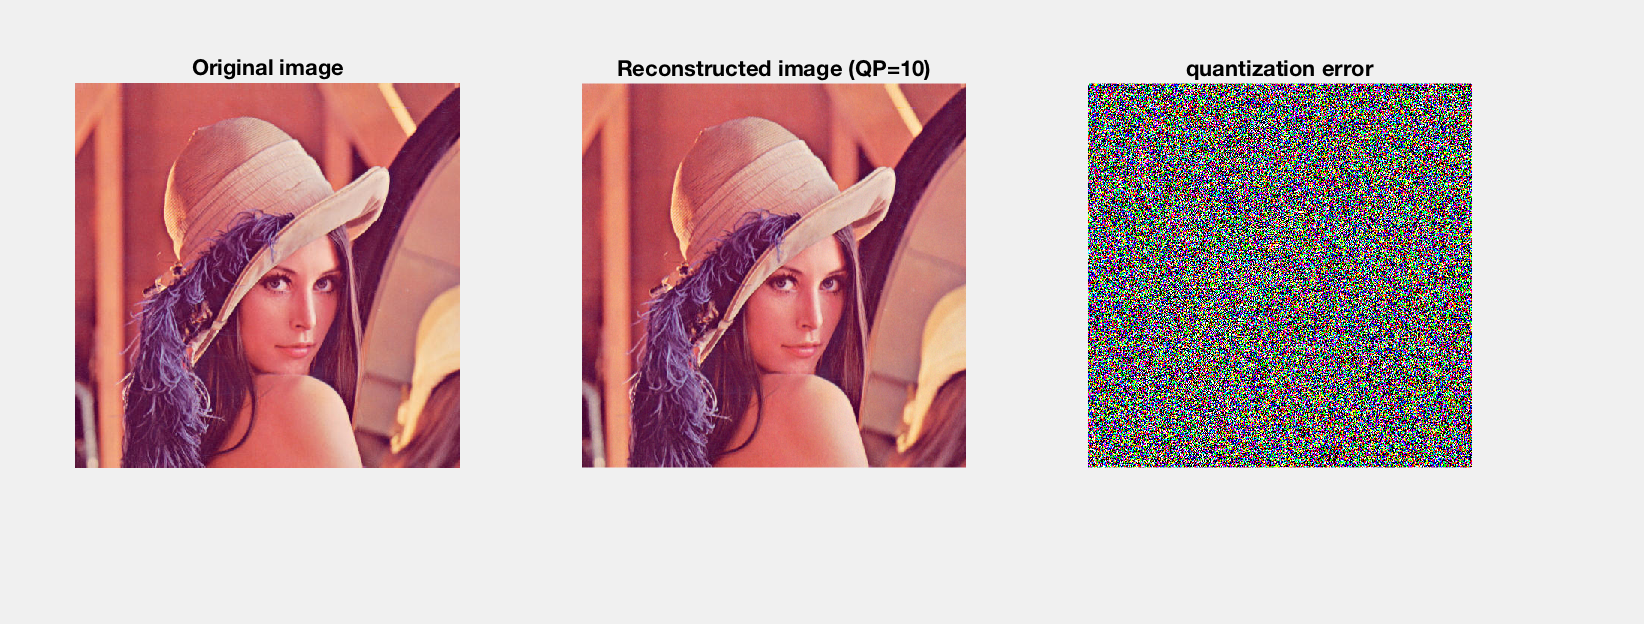
\includegraphics[height=0.4\textwidth]{./img/quant.png}
\caption{Quantization}
\end{figure}

\newpage


\section{Assignment 9 Motion estimation}
\label{sec:org80e6a1e}
\subsection{Apply quantization error on MC prediction error}
\label{sec:org1d8ee8a}
\begin{verbatim}
pf(r:r+N-1,c:c+N-1) = B1(r+N:r+N2-1,c+N:c+N2-1)-A1(r+N+y1:r+y1+N2-1,c+N+x1:c+x1+N2-1);
temp = pf(r:r+N-1,c:c+N-1);
TemP = dct2(temp); % DCT of difference
s = sign(TemP); % extract the coefficient sign
TemP = s .* round(abs(TemP)/8)*8; % quantize/dequantize DCT
temp = idct2(TemP); % IDCT
Br_quant(r:r+N-1,c:c+N-1) = A1(r+N+y1:r+y1+N2-1,c+N+x1:c+x1+N2-1)+ temp;
\end{verbatim}

\subsection{Question a}
\label{sec:orgade3232}

\begin{verbatim}
   x = int16(zeros(Height/N,Width/N));% x-component of motion vector
y = int16(zeros(Height/N,Width/N));% y-component of motion vector
x(rblk,cblk) = v; y(rblk,cblk) = u;
\end{verbatim}

x stores x coordinate of motion vector, y stores y coordinate of motion vector.

\subsection{Question b}
\label{sec:orgba33989}
The size of image is 176 * 144
So the total number of motion vector will be: $$\frac{176}{8}\times\frac{144}{8} = 22 \times 18 = 396$$

\subsection{Question c}
\label{sec:orgece9221}
The motion compensated frame stoed in Pr which abstract out the best match block in reference frame.
\begin{verbatim}
pf(r:r+N-1,c:c+N-1) = B1(r+N:r+N2-1,c+N:c+N2-1)-A1(r+N+y1:r+y1+N2-1,c+N+x1:c+x1+N2-1);
\end{verbatim}



\newpage
\section{Assignment 10}
\label{sec:org33cff40}

\begin{enumerate}
\item Uncomment \% A=transpose(A);  line 26
\item Uncomment \% B=transpose(B);  line 63
\item The image size normaliztion is incorrect.
\end{enumerate}
\begin{verbatim}
% Make image size divisible by 16
[X,Y] = size(A);
if mod(X,16)~=0
    Height = floor(X/16)*16;
else
    Height = X;
end
if mod(Y,16)~=0
    Width = floor(Y/16)*16;
else
    Width = Y;
end
\end{verbatim}

change to 8 as

\begin{verbatim}
% Make image size divisible by 8
[X,Y] = size(A);
if mod(X,8)~=0
    Height = floor(X/16)*16;
else
    Height = X;
end
if mod(Y,8)~=0
    Width = floor(Y/16)*16;
else
    Width = Y;
end

\end{verbatim}

line 23

\begin{enumerate}
\item change inFile1='table\(_{\text{40.raw}}\)'; to 'table\(_{\text{39.raw}}\)' line 23
\item change F = int16(41:43); to F = int16(40:43); line 50
\item change legend('MC','No MC', 0) to legend('MC','No MC', 'best') line 114
\item change legend('MC','No MC', 0) to legend('MC','No MC', 'best') line 118
\end{enumerate}


\newpage

\section{Assignment 11 Stereo Imaging}
\label{sec:org9ab7902}

The larger the factor the lower offset generate for red and blue image.

Original : D = round(Y2\{nf\}/2);  \%adjust depth factor '2'

Modify To : D = round(Y2\{nf\}/5);
\end{document}